% =====================================================================
\section{Geometry of the Gradient}\label{ch:geometry}
% =====================================================================

The slides prove that $\grad f$ points in the direction of fastest increase.
This chapter adds the companion fact that makes gradients so useful in
geometry: the gradient is \emph{perpendicular to level curves and level
surfaces}. It explains Figure~\ref{fig:trio} and gives a quick way to find
tangent lines and tangent planes. (This material extends the slides; it is
standard in the course textbook and frequently appears as part of a gradient
problem.)

\subsection{The gradient is perpendicular to level curves}

\begin{theorem}\label{thm:grad-perp}
Let $f$ be differentiable and let $P(x_0,y_0)$ lie on the level curve
$f(x,y)=k$. If $\grad f(x_0,y_0)\neq\vzero$, then $\grad f(x_0,y_0)$ is
perpendicular to the level curve at $P$, i.e.\ to its tangent vector.
The same holds in three variables: $\grad f(x_0,y_0,z_0)$ is normal to the
level surface $f(x,y,z)=k$ through the point.
\end{theorem}

\begin{proof}
Let $\vr(t)=\ip{x(t),y(t)}$ be a differentiable parametrization of the level
curve with $\vr(t_0)=\ip{x_0,y_0}$. Since the curve lies in the level set,
$f(x(t),y(t))=k$ for all $t$. Differentiate both sides with respect to $t$
using the chain rule (Theorem~\ref{thm:chain}):
\[
  f_x\,x'(t)+f_y\,y'(t)=0,\qquad\text{i.e.}\qquad \grad f(\vr(t))\cdot\vr\,'(t)=0 .
\]
At $t=t_0$ this says $\grad f(x_0,y_0)\perp\vr\,'(t_0)$, the tangent vector.
For a level surface, apply the same argument to every curve on the surface
through the point: $\grad f$ is perpendicular to all their tangent vectors,
hence to the tangent plane.
\end{proof}

Combined with Theorem~\ref{thm:max}, this gives the familiar picture of a
contour map (Figure~\ref{fig:contour-gradient}): gradient vectors cross the
level curves at right angles, pointing ``uphill'', and they are longest where
the level curves are packed most tightly (where the surface is steepest).

\begin{figure}[H]
  \centering
  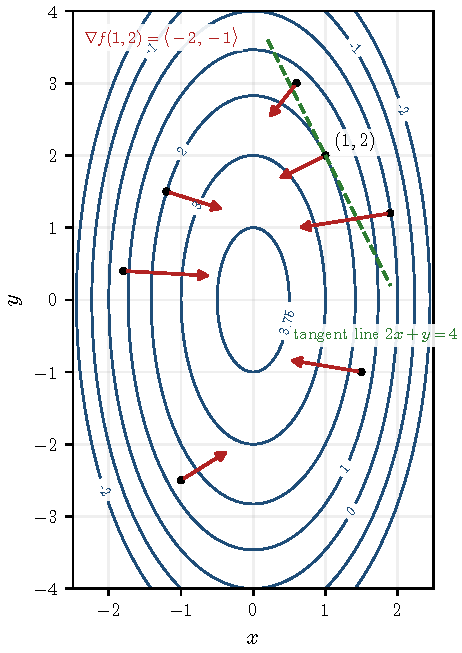
\includegraphics[width=0.62\linewidth]{contour_gradient}
  \caption{Level curves of $f(x,y)=4-x^2-\frac14y^2$ (labelled with their
  heights) and gradient vectors $\grad f=\ip{-2x,-\frac y2}$ (red, scaled by
  $0.35$). Each gradient is perpendicular to the level curve through its base
  point and points toward higher values. Green: the tangent line at $(1,2)$
  found in Example~\ref{ex:tangent-line}.}
  \label{fig:contour-gradient}
\end{figure}

\begin{example}[Tangent line to a level curve]\label{ex:tangent-line}
Find the tangent line at $(1,2)$ to the level curve of
$f(x,y)=4-x^2-\tfrac14y^2$ that passes through that point.
\end{example}
\begin{solution}
\step{1}{Which level curve?} $f(1,2)=4-1-1=2$, so the curve is
$4-x^2-\tfrac14y^2=2$, i.e. $x^2+\frac{y^2}{4}=2$.
\step{2}{Normal vector.} $\grad f(1,2)=\ip{-2(1),-\tfrac12(2)}=\ip{-2,-1}$ is
perpendicular to the curve at $(1,2)$.
\step{3}{Line through $(1,2)$ perpendicular to $\ip{-2,-1}$.}
\[
  -2(x-1)-1(y-2)=0\iff 2x+y=4 .
\]
\step{4}{Check by implicit differentiation.} $2x+\frac{y}{2}y'=0\Rightarrow
y'=-\frac{4x}{y}=-2$ at $(1,2)$, the slope of $y=4-2x$.\checkok
\end{solution}

\subsection{Tangent planes and normal lines to level surfaces}

\begin{definition}
Let $S$ be the level surface $F(x,y,z)=k$ and $P(x_0,y_0,z_0)$ a point of $S$
with $\grad F(P)\neq\vzero$.
\begin{itemize}
\item The \emph{tangent plane} to $S$ at $P$ is the plane through $P$ with
      normal vector $\grad F(P)$:
      \[
        F_x(P)(x-x_0)+F_y(P)(y-y_0)+F_z(P)(z-z_0)=0 .
      \]
\item The \emph{normal line} to $S$ at $P$ is the line through $P$ in the
      direction of $\grad F(P)$:
      \[
        x=x_0+F_x(P)\,t,\quad y=y_0+F_y(P)\,t,\quad z=z_0+F_z(P)\,t .
      \]
\end{itemize}
\end{definition}

\begin{example}[Tangent plane to an ellipsoid]\label{ex:ellipsoid}
Find the equations of the tangent plane and normal line at $(-2,1,-3)$ to the
ellipsoid $\dfrac{x^2}{4}+y^2+\dfrac{z^2}{9}=3$.
\end{example}
\begin{solution}
\step{1}{Set up $F$.} $F(x,y,z)=\dfrac{x^2}{4}+y^2+\dfrac{z^2}{9}$; the ellipsoid is
the level surface $F=3$. Check the point: $\frac44+1+\frac99=3$.\checkok
\step{2}{Gradient.} $\grad F=\ip{\dfrac x2,\;2y,\;\dfrac{2z}{9}}$, so
$\grad F(-2,1,-3)=\ip{-1,\;2,\;-\tfrac23}$.
\step{3}{Tangent plane.}
\[
  -1(x+2)+2(y-1)-\tfrac23(z+3)=0 .
\]
Multiplying by $-3$: $3(x+2)-6(y-1)+2(z+3)=0$, i.e.
$\boxed{3x-6y+2z+18=0}$.
\step{4}{Normal line.} $x=-2-t,\quad y=1+2t,\quad z=-3-\tfrac23t$.
\end{solution}

\begin{figure}[H]
  \centering
  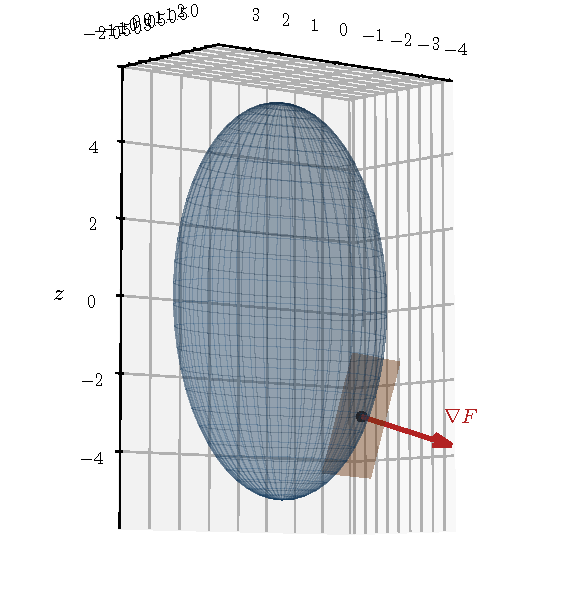
\includegraphics[width=0.5\linewidth]{ellipsoid_tangent_plane}
  \caption{The ellipsoid of Example~\ref{ex:ellipsoid}, a patch of its tangent
  plane at $(-2,1,-3)$, and the normal vector $\grad F(-2,1,-3)$.}
  \label{fig:ellipsoid}
\end{figure}

\begin{remark}[Graphs are level surfaces]
The graph $z=f(x,y)$ is the level surface $F(x,y,z)=f(x,y)-z=0$, and
$\grad F=\ip{f_x,f_y,-1}$. The tangent plane at $(x_0,y_0,z_0)$ is therefore
$f_x(x-x_0)+f_y(y-y_0)-(z-z_0)=0$, i.e.
\[
  z-z_0=f_x(x_0,y_0)(x-x_0)+f_y(x_0,y_0)(y-y_0),
\]
the usual tangent-plane formula for a graph.
\end{remark}

\begin{example}\label{ex:tp-graph}
Find the tangent plane to $z=4-x^2-\frac14y^2$ at $(1,2,2)$.
\end{example}
\begin{solution}
$f_x(1,2)=-2$, $f_y(1,2)=-1$, so $z-2=-2(x-1)-1(y-2)$, i.e. $2x+y+z=6$.
(Check: $2+2+2=6$.\checkok) Notice that the tangent line of
Figure~\ref{fig:surface-slice} lies in this plane: its points
$\left(1+\frac t2,\;2+\frac{\sqrt3}{2}t,\;2-\left(1+\frac{\sqrt3}{2}\right)t\right)$
satisfy $2x+y+z=6$ for every $t$.
\end{solution}

\subsection{Paths of steepest ascent}

A hiker who always walks in the direction of the gradient follows a
\emph{path of steepest ascent}. Its projection onto the $xy$-plane is a curve
whose tangent is parallel to $\grad f$ at every point, so it crosses every
level curve at right angles.

\begin{example}\label{ex:steepest}
For the hill $z=4-x^2-\frac14y^2$, find the path of steepest ascent (in the
$xy$-plane) starting at $(1,2)$.
\end{example}
\begin{solution}
\step{1}{Slope condition.} A curve $y=y(x)$ has tangent direction
$\ip{1,y'}$, which must be parallel to $\grad f=\ip{-2x,-\frac y2}$. Hence
\[
  \frac{\dd y}{\dd x}=\frac{f_y}{f_x}=\frac{-y/2}{-2x}=\frac{y}{4x}.
\]
\step{2}{Separate variables} (for $x,y>0$):
$\displaystyle\int\frac{\dd y}{y}=\int\frac{\dd x}{4x}\Rightarrow\ln y=\tfrac14\ln x+C
\Rightarrow y=Kx^{1/4}.$
\step{3}{Initial point.} $2=K\cdot1^{1/4}$, so $K=2$ and the path is
$y=2x^{1/4}$, travelled from $(1,2)$ toward the summit $(0,0)$ (the gradient
$\ip{-2,-1}$ at the start points toward decreasing $x$).
\end{solution}

\begin{figure}[H]
  \centering
  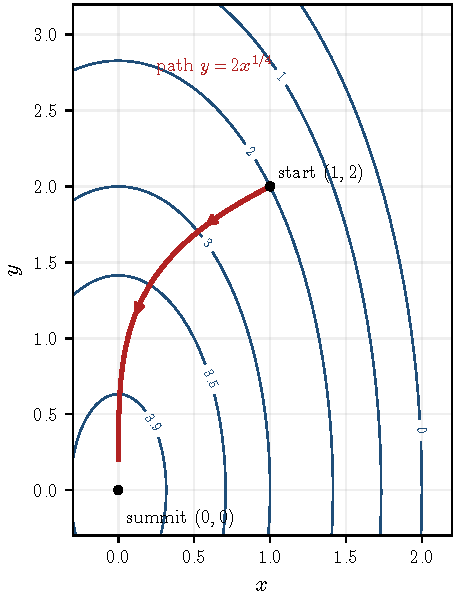
\includegraphics[width=0.48\linewidth]{steepest_ascent}
  \caption{The path of steepest ascent $y=2x^{1/4}$ from $(1,2)$ crosses every
  level curve at a right angle and climbs to the summit.}
  \label{fig:steepest}
\end{figure}

\subsection{What the gradient tells you}

\begin{center}
\renewcommand{\arraystretch}{1.35}
\begin{tabularx}{0.95\linewidth}{>{\raggedright\arraybackslash}p{0.38\linewidth}X}
\toprule
\textbf{Question at a point $P$} & \textbf{Answer in terms of $\grad f(P)$}\\
\midrule
Rate of change in direction $\vu$ ($\norm{\vu}=1$) & $\Du f(P)=\grad f(P)\cdot\vu$\\
Direction of fastest increase & $\grad f(P)$ \quad (unit: $\grad f/\norm{\grad f}$)\\
Fastest rate of increase & $\norm{\grad f(P)}$\\
Direction / rate of fastest decrease & $-\grad f(P)$, \ rate $-\norm{\grad f(P)}$\\
Directions of zero rate & $\vu\perp\grad f(P)$ (tangent to the level curve)\\
Normal to level curve / surface & $\grad f(P)$\\
Possible values of $\Du f(P)$ & exactly $\left[-\norm{\grad f(P)},\,\norm{\grad f(P)}\right]$\\
\bottomrule
\end{tabularx}
\end{center}
